\documentclass{scrartcl}

\usepackage{ucs}
\usepackage[utf8x]{inputenc}
\usepackage[english]{babel}
\usepackage{graphicx}
\usepackage{amsmath}
\usepackage{amssymb}
\usepackage{mathtools}
\usepackage{titlesec}
\usepackage{xcolor}
\usepackage{listings}

\DeclarePairedDelimiter\abs{\lvert}{\rvert}%
\DeclarePairedDelimiter\norm{\lVert}{\rVert}%

% Swap the definition of \abs* and \norm*, so that \abs
% and \norm resizes the size of the brackets, and the 
% starred version does not.
\makeatletter
\let\oldabs\abs
\def\abs{\@ifstar{\oldabs}{\oldabs*}}
%
\let\oldnorm\norm
\def\norm{\@ifstar{\oldnorm}{\oldnorm*}}
\makeatother

\setcounter{secnumdepth}{4}

\titleformat{\paragraph}
{\normalfont\normalsize\bfseries}{\theparagraph}{1em}{}
\titlespacing*{\paragraph}
{0pt}{3.25ex plus 1ex minus .2ex}{1.5ex plus .2ex}

\setlength\parindent{0pt}

\lstset{ %
	language=Java,
	frame=single,
	showspaces=false,
	showtabs=false,
	breaklines=true,
	showstringspaces=false,
	breakatwhitespace=true,
	commentstyle=\color{green},
	keywordstyle=\color{blue},
	stringstyle=\color{red},
	basicstyle=\ttfamily,
}

\title{Grundlagen des Compilerbau \\ Zusammenfassung}
\author{Thomas Mohr}
\date{}

\begin{document}
\maketitle
\pagebreak
\tableofcontents
\pagebreak

\section{Introduction}

\subsection{Language Processors}

\begin{itemize}
	\item Compilers are programs that
	\begin{itemize}
		\item read programs in source language
		\item produce equivalent programs in target language
		\item report errors encountered during translation
	\end{itemize}
	\begin{figure}[ht!]
		\centering
		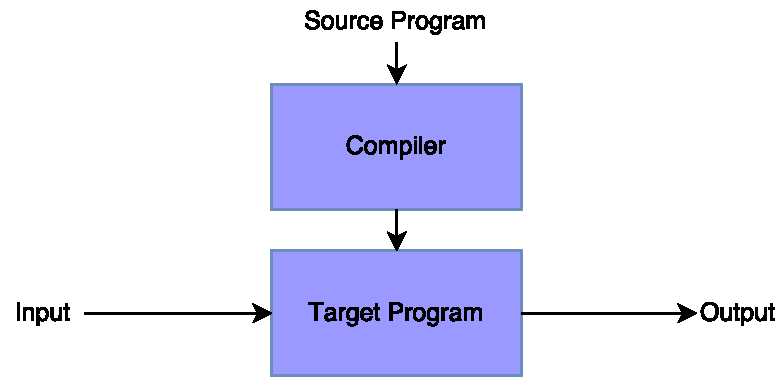
\includegraphics[width=0.7\linewidth]{figures/compilers}
		\caption{Compiler}
		\label{fig:compilers}
	\end{figure}
	\item Interpreters are programs that
	\begin{itemize}
		\item read programs in source language
		\item read input
		\item directly perform operations of source programs
	\end{itemize}
	\begin{figure}[ht!]
		\centering
		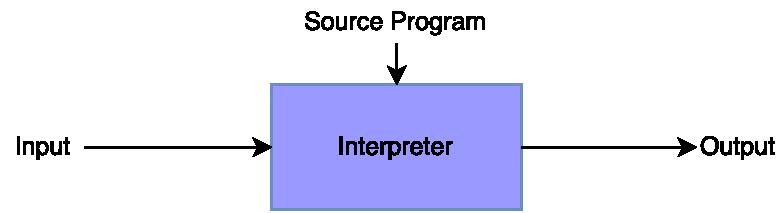
\includegraphics[width=0.7\linewidth]{figures/interpreters}
		\caption{Interpreter}
		\label{fig:interpreters}
	\end{figure}
	\item In hybrid approaches
	\begin{itemize}
		\item compiler first generates intermediate code, not directly executable on physical machine
		\item interpreter processes intermediate code
	\end{itemize}
	\begin{figure}[ht!]
		\centering
		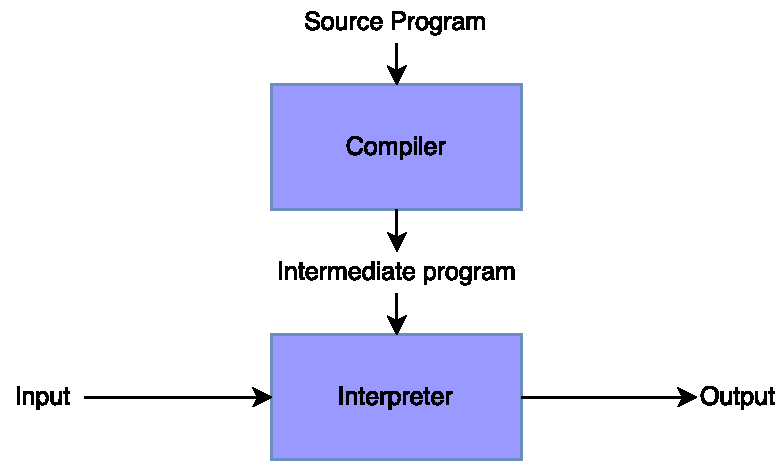
\includegraphics[width=0.7\linewidth]{figures/in_hybrid_processors}
		\caption{Hybrid}
		\label{fig:inhybridprocessors}
	\end{figure}
\end{itemize}

\subsection{Compiler Phases}

\begin{figure}[ht!]
	\centering
	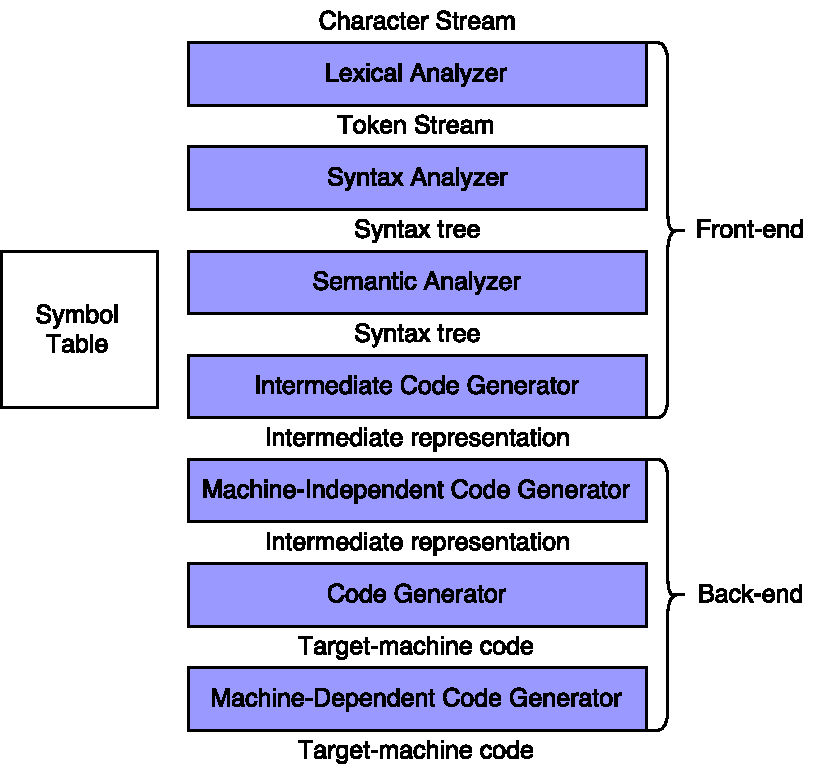
\includegraphics[width=0.7\linewidth]{figures/anatomy_of_a_compiler}
	\caption{Anatomy of a Compiler}
	\label{fig:anatomyofacompiler}
\end{figure}


\subsubsection{Lexical Analysis or Scanning}

\begin{itemize}
	\item Read character stream
	\item Group characters into lexemes
	\begin{itemize}
		\item Meaningful to compiler
		\item Has token name and attribute values
	\end{itemize}
	\item Examples
	\begin{itemize}
		\item $ 60: \langle \text{integer}, 60 \rangle $
		\item $ \text{new}: \langle \text{keyword} \rangle $
		\item $ \text{setValue}: \langle \text{identifier},\text{'setValue'} \rangle $
	\end{itemize}
\end{itemize}

\subsubsection{Syntax Analysis or Parsing}

\begin{itemize}
	\item Arrange tokens in trees
	\item Representing grammatical structure of program
	\item Disambiguates possible meanings (e.g. operator precedence)
\end{itemize}

\subsubsection{Semantic Analysis}

\begin{itemize}
	\item The grammar generally allows writing more programs than are meaningful
	\begin{itemize}
		\item Using stricter grammar would exclude too many meaningful programs
		\item Semantic analysis checks whether program can be executed
	\end{itemize}
	\item For example:
	\begin{itemize}
		\item Are value types of operands compatible?
		\item Are identifiers used that refer to applicable program element?
	\end{itemize}
	\item Gather type information in symbol table
\end{itemize}

\subsubsection{Intermediate Code Generation}

\begin{itemize}
	\item Optionally generate intermediate code
	\item Properties
	\begin{itemize}
		\item Easy to generate
		\item Easy to translate to target machine code
		\item Easy to optimize
	\end{itemize}
\end{itemize}

\subsubsection{Code Optimization}

\begin{itemize}
	\item Improve intermediate code
	\begin{itemize}
		\item Faster
		\item Shorter
		\item Consuming less energy
	\end{itemize}
	\item E.g., statically evaluate sub expressions
\end{itemize}

\subsubsection{Code Generation}

\begin{itemize}
	\item Only truly machine-specific phase
	\item Map intermediate code operations to physical machine operations
	\begin{itemize}
		\item Possibly exploit special-purpose instructions
		\item Map variables to registers or other locations
	\end{itemize}
\end{itemize}

\subsection{Symbol Table Management}

\begin{itemize}
	\item Maintain information on visible symbols
	\begin{itemize}
		\item Name
		\item Type
		\item Signature of procedures
	\end{itemize}
	\item Variables have a scope
	\begin{itemize}
		\item Global
		\item Local
		\item Nested scopes
	\end{itemize}
	\item Symbol table shared among all phases
\end{itemize}

\subsection{Environment}

\begin{itemize}
	\item Rules for determining location corresponding to name
	\item Resolution depends on different factors
	\begin{itemize}
		\item Kind of program element referenced by name
		\item Programming language design
	\end{itemize}
	\item Generally determined by two policies
	\begin{itemize}
		\item Binding (find location for name)
		\item Scoping (find correct decleration for name)
	\end{itemize}
\end{itemize}

\subsubsection{Binding}

\begin{itemize}
	\item Bind name to location
	\item Static (location is always the same for each appearance of name)
	\item Dynamic (location may be different each time name is used)
	\item Binding most commonly is dynamic
\end{itemize}

\subsubsection{Scoping}

\begin{itemize}
	\item Range of validity for name decleration
	\begin{itemize}
		\item Where can a declared name be used?
		\item Upon usage of name: Which is the decleration it refers to?
	\end{itemize}
	\item Strategies
	\begin{itemize}
		\item Static scoping
		\begin{itemize}
			\item Sequence of top-level declerations of variables and functions
			\begin{itemize}
				\item Valid until end of program
			\end{itemize}
			\item Functions start with sequence of local variable declerations
			\begin{itemize}
				\item Valid until end of function
				\item Shadow global declerations with same name
			\end{itemize}
		\end{itemize}
		\item Block structure
		\begin{itemize}
			\item Block is specific kind of instruction
			\item Start by sequence of declerations
			\item Followed by statements
			\item Decleration shadows declerations in outer blocks/function/global scope
		\end{itemize}
		\item Dynamic scoping
		\begin{itemize}
			\item Scope determined at runtime
			\item Decleration is valid from the moment it is encountered at runtime
		\end{itemize}
	\end{itemize}
\end{itemize}

\subsection{Parameter Passing}

\begin{itemize}
	\item Call-by-value
	\begin{itemize}
		\item Value of variable is copied before procedure call
		\item Expressions are evaluated into temporary variable first
		\item Procedure gets own storage location for each parameter
		\item Can be costly for large data types
		\item Example (Main): $ 2*2-4*1*3=-8 $
	\end{itemize}
	\item Call-by-reference
	\begin{itemize}
		\item Reference to storage location is passed to procedure
		\item Can modify value of variable from caller
	\end{itemize}
	\item Call-by-name
	\begin{itemize}
		\item Pass full expressions to procedure
		\item Evaluate in place where formal parameter is used
		\item Example (Main): $ 1*2-4*3*4=-46 $
	\end{itemize}
\end{itemize}

\begin{lstlisting}
class Main {
    int index = 0;
    int[] arr = {0,1,2,3,4,5};
    
    int discr(int a, int b, int c) {
        int value = b * b - 4 * a * c;
        return value;
    }

    int arrNext() {
    	index++;
    	return arr[index];
    }

    public static void main(String... args) {
    	System.out.print(discr(
    	    arrNext(), 
    	    arrNext(), 
    	    arrNext()
    	));
    }
}
\end{lstlisting}

\subsection{Aliasing}

\begin{itemize}
	\item Call-by-reference semantic can lead to aliases
	\item Aliases prevent optimizations
	\begin{itemize}
		\item Assume local variable has single assignment
		\item Optimization could replace occurence of variable with constant
		\item If aliases exist for variable, undetected changes may occur and therefore optimization may be incorrect
	\end{itemize}
\end{itemize}

\pagebreak
\section{Lexical Analysis}

\subsection{Scanner}

\begin{itemize}
	\item Definitions
	\begin{itemize}
		\item $ \Sigma $: Input alphabet
		\item $ p \in \Sigma^* $: Input
		\item $ L \in \mathcal{P} $: Language
	\end{itemize}
	\item Tasks
	\begin{itemize}
		\item Split source program into sequence of lexemes
		\item Transform sequence of lexemes to sequence of tokens
	\end{itemize}
	\item Many different lexemes play the same role
	\begin{itemize}
		\item Group into classes of lexemes: tokens
		\item Token: $ \langle \text{token-name, attribute(s)} \rangle $
	\end{itemize}
\end{itemize}

\subsection{Typical kinds of Tokens}

\begin{itemize}
	\item Identifiers
	\begin{itemize}
		\item Sequence of letters and digits
		\item Start with letter
	\end{itemize}
	\item Numbers
	\begin{itemize}
		\item Sequence of digits
		\item Possibly with a sign
	\end{itemize}
	\item Keywords
	\item Special characters
	\begin{itemize}
		\item Operators: $ +,*,\ldots $
		\item Parantheses: $ (,),\{,\} $
		\item $ \ldots $
	\end{itemize}
	\item Compund symbols
	\begin{itemize}
		\item Operators: $ ==,<=,++,\ldots $
	\end{itemize}
	\item Whitespace
	\begin{itemize}
		\item Space
		\item Tab
		\item Newline
		\item $ \ldots $
	\end{itemize}
	\item Special symbols
	\begin{itemize}
		\item Comments
		\item Pragmas (Compiler Anweisungen)
	\end{itemize}
\end{itemize}

\subsection{Regular Expressions}

\begin{itemize}
	\item $ RE(\Sigma) $: Regular Expression
	\begin{itemize}
		\item $ \epsilon \in RE(\Sigma) $: The empty expression
		\item $ \forall a \in \Sigma.a \in RE(\Sigma) $: All characters of $ \Sigma $
		\item Given $ \alpha,\beta \in RE(\Sigma) $
		\begin{itemize}
			\item $ (\alpha \vert \beta) \in RE(\Sigma) $
			\item $ (\alpha \cdot \beta) \in RE(\Sigma) $
			\item $ (\alpha^*) \in RE(\Sigma) $
		\end{itemize}
		\item Closed under regular composition
		\item Order of precedence: $ *,\cdot,\vert $
	\end{itemize}
	\item $ [[RE(\Sigma)]] $: Language generated by regular expression
	\begin{itemize}
		\item $ [[\epsilon]] := \emptyset $
		\item $ [[\alpha]] := \{\{a\}\vert \forall a \in \Sigma\} $
		\item $ [[\alpha\vert\beta]] := [[\alpha]] \cup [[\beta]] $
		\item $ [[\alpha\cdot\beta]] := [[\alpha]]\cdot[[\beta]] $ (element-wise concatenation)
		\item $ [[\alpha^*]] := [[\alpha]]^* $ (closure)
		\item $ [[\epsilon^*]] := \{\epsilon\} $
	\end{itemize}
\end{itemize}

\subsection{Non-Deterministic Finite Automaton}


	
\end{document}